\section{Introduction}

In recent years, the computer vision field has converged on a general method for object detection, and a standard evaluation of results.
Most current state-of-the-art object detection systems consist of three tasks: proposing regions of the image, evaluating a given region for presence of an object of a given category, and post-processing the results.
In the evaluation ground truth, each object is most commonly assumed to belong to one of a fixed set of classes; its location is approximated by placing a bounding box around pixels belonging to it.
Large datasets of such human annotations are used for evaluation of detection algorithms~\cite{pascal-voc-2010,imagenet_cvpr09}.

With few exceptions, current detection systems are not inherently multi-class.
Instead, separate detectors are trained per class, and they are deployed and evaluated independently.
The evaluation of multi-class performance, if at all given, consists of averaging the per-class metrics.
Some notable papers do make multi-class detection a priority, and accordingly evaluate in a multi-class setting, where false positives can be generated both by incorrect localization and incorrect labeling.
State-of-the-art detection systems also do not generally make efficiency a goal.

\begin{figure}[ht!]
\center{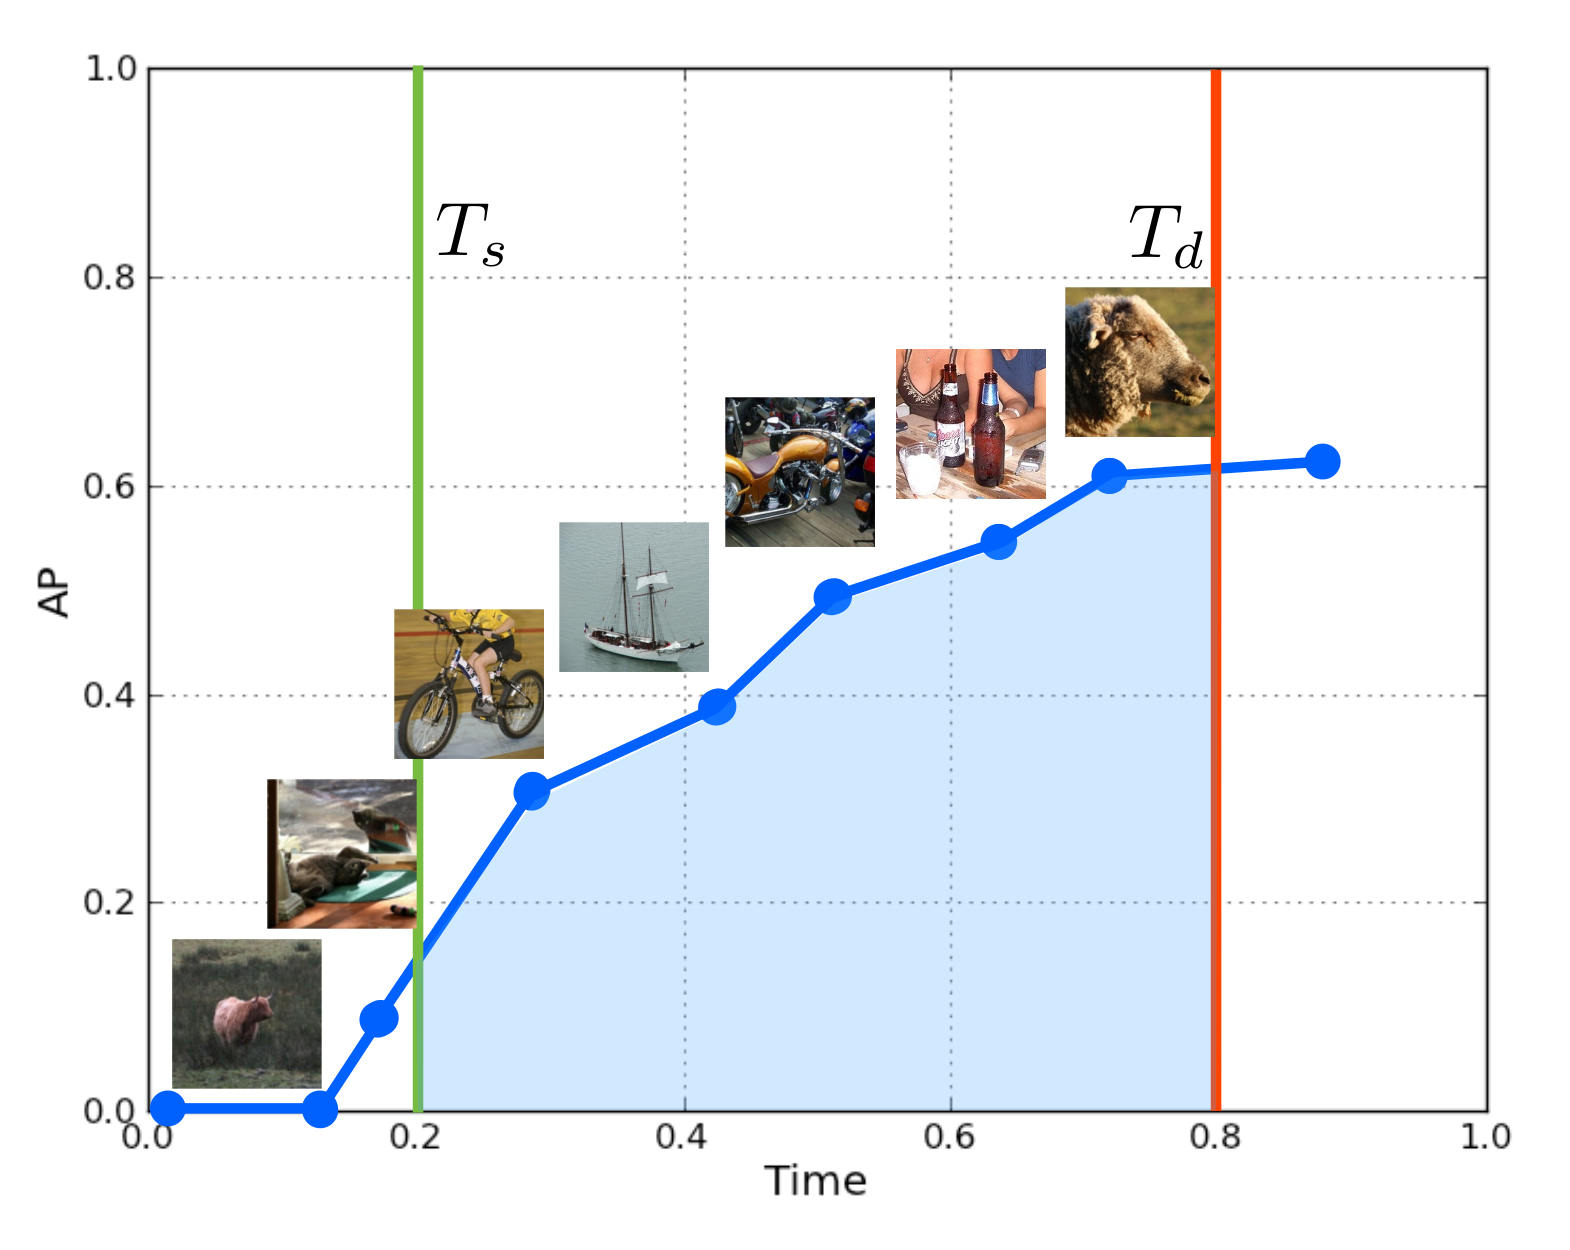
\includegraphics[width=0.56\linewidth]
    {../figures/evaluation_thumbs.png}}
  \caption{We aim for \emph{Anytime} performance within the bounds of the curve. That is, the policy should give the best possible answer at any time from start time $T_s$ to deadline $T_d$.}
  \label{fig:evaluation}
\end{figure}

It is of course important to refrain from locking object recognition research into a single detector architecture with a focus only on increasing efficiency.
That said, there are applications for which performance truly is time-sensitive.
In robotics, a small finite amount of processing power per unit time is all that is available for robust object detection if the robot is to usefully interact with humans.
In large-scale detection system deployments, such as for image search, results need to be obtained quickly per image as the number of images to process is large and growing.
When processing large photo collection on end-user machines for immediate consumer navigation, the same is true.

In all these cases, an acceptable answer at a reasonable time may be more valuable than the best answer given too late.
Furthermore, the value of the answer depends largely on the target application.

A hypothetical recognition system for a vision-based advertising deployment presents a case study.
The system will have different accuracies for objects of different classes; detections will have different values based on confidence and class; and the queue of unprocessed images will vary in size.
The most rational detection strategy in such an environment should depend on all of these variables.

We argue that the key to tackling such problems of dynamic recognition resource allocation is to start asking a new question:
\emph{What is the best performance we can get on a budget?}
To answer it, we consider the evaluation metric of performance vs. time, shown in Figure~\ref{fig:evaluation} and discussed further in the text.
Our goal is a dynamic policy for selecting classifiers or detectors to achieve the highest recognition performance under this evaluation.
